% SPDX-License-Identifier: GPL-2.0-or-later

% Copyright 2022 Association Prologin <info@prologin.org>

%LaTeX Document
\documentclass[a4paper,twoside,12pt]{article}
\usepackage{xltxtra}
\usepackage{url}
\usepackage{caption}
%\usepackage{lettrine}
\usepackage{amssymb}
\usepackage{wrapfig}
\usepackage{longtable}
\usepackage{booktabs}
\usepackage{hyperref}
\setromanfont[Mapping=tex-text]{TeX Gyre Pagella}
\setsansfont[Mapping=tex-text]{DejaVu Sans}
\setmonofont[
  Mapping=tex-text,
%  Scale=0.85,
  AutoFakeSlant,
  BoldItalicFeatures={FakeSlant}]{Inconsolata}
%\newfontfamily{\A}[Scale=0.85]{DejaVu Sans} % TODO find a free Arial/Helvetica equivalent
%\newfontfamily{\J}[Scale=0.85]{Hiragino Kaku Gothic Pro}
%\newfontfamily{\P}[Scale=0.85]{Palatino}
\usepackage{soul} % Pour barrer
\usepackage{textcomp} % Pour les trademarks


\usepackage{cellspace}
\setlength\cellspacetoplimit{4pt}
\setlength\cellspacebottomlimit{4pt}
\newcommand\cincludegraphics[2][]{\raisebox{-0.2\height}{\includegraphics[#1]{#2}}}

%%%%%%%%%%%%%%%%%%%%%%%%%%%%%%%%
%%         BEGIN FIXME         %
%%%%%%%%%%%%%%%%%%%%%%%%%%%%%%%%
\def\plongday{Vendredi}
\def\pday{27}
\def\pmonth{Mai}
\def\pyear{2022}

\def\ptitle{\textsc{La baguette légendaire}} %% Subject's main title
\def\psubtitle{La marche des canards} %% Subject's sub title

\def\plogo{img/logo2022.png} %% Logo FIXME
\def\psubjectpicture{img/logo-finale-2022.png} %% Picture to be displayed FIXME

%% on its own page \vspace*{0.1cm}}
%%%%%%%%%%%%%%%%%%%%%%%%%%%%%%%%
%%         END FIXME           %
%%%%%%%%%%%%%%%%%%%%%%%%%%%%%%%%

%%%%%%%%%%%%%%%%%%%%%%%%%%%%%%%%%%%%%%%%%%%%%%%%%%%%%%%%
%%              DO NOT EDIT PAST THIS LINE            %%
%%%%%%%%%%%%%%%%%%%%%%%%%%%%%%%%%%%%%%%%%%%%%%%%%%%%%%%%


%\documentclass[a4paper,twoside,12pt]{book}

\usepackage[french]{babel} % TODO switch to polyglossia?
\usepackage{geometry}
\usepackage{multicol}
\usepackage{fancyhdr}
\usepackage{listings}
\usepackage{array}
\usepackage{color}
\usepackage{caption}
\usepackage{subcaption}
\usepackage{amsmath}
\usepackage{tikz}

\def\pdate{\plongday{} \pday{} \pmonth{} \pyear{}}
\def\tightlist{} % fix for pandoc

\definecolor{colIdentifier}{gray}{0}
\definecolor{colKeys}{rgb}{0,0,0.6}
\lstset{
    extendedchars=false,
    showstringspaces=false,
    escapeinside=@@,
%    keywordstyle=\color{blue},
%    commentstyle=\color[rgb]{0.133,0.545,0.133},
    columns=flexible,
    language=C++,
    tabsize=2,
    basicstyle=\ttfamily\NoAutoSpacing
%    numbers=left,
%    frame=lines
}
\lstnewenvironment{lst-c++}{%
\lstset{%
  breaklines=true,
  postbreak=\mbox{\textcolor{red}{$\hookrightarrow$}\space},
  language=C++
}}{}

\newcommand{\wfig}[2]{
}


\captionsetup{justification=centering}

%\renewcommand\ttdefault{cmtt}

\newcommand{\functitle}[1]{%
\vspace{0.5cm}
$\bullet$ \underline{\textbf{#1}}
}

%\NoAutoSpaceBeforeFDP
\geometry{bindingoffset=5mm,hmarginratio=1:1,heightrounded,headheight=15pt,bmargin=3cm}

\setcounter{tocdepth}{2}

\makeindex

\begin{document}
\pagestyle{empty}
\sloppy

\lhead[\thepage]{\nouppercase \leftmark}
\rhead[\textsl{Prologin \pyear{}} --- Sujet de la finale]{\thepage}
%%\cfoot{\color{red}TOP SECRET//SI//ORCON//NOFORN}

\sethlcolor{black}

% Couverture =========================================================
\begin{titlepage}
\begin{center}
~\includegraphics[width=\linewidth]{\plogo}\\
\vspace{5cm}
\Huge
\textbf{\ptitle{}}

\vspace{1cm}

\Large
\textbf{\psubtitle{}}

\vspace{2cm}

\normalsize
\textnormal Sujet de la finale du Concours National d'Informatique\\
\pdate\\

\end{center}


\end{titlepage}

\small

% Sommaire ===========================================================
\cleardoublepage
\tableofcontents

\normalsize

% Corps ==============================================================
%\cleardoublepage
\setcounter{page}{1}
\pagestyle{fancy}
\parskip=6pt plus 3pt

\newpage
\vspace{4cm}
\begin{center}\includegraphics[height=14cm]{\psubjectpicture}\end{center}

\pagebreak

\section{Contexte} % on peut changer "Contexte" pour autre chose

% Bravo et Félicitations ...

\textbf{\large La baguette}

% Côté RP du concours

Inscrite profondément dans la culture française, la baguette prend
place dans de nombreux foyers chaque jour. Tartinée de confiture le
matin, surplombée de fromage le midi et baignant dans la soupe le soir,
ce pain a su conquérir et ravir les Humains.

% https://www.franceculture.fr/gastronomie/a-lorigine-de-la-baguette-de-pain

3 légendes entourent sa création. Certains affirment que c'est sous
les boulangers de Napoléon, au début du XIX$^{\text{ème}}$ siècle qu'elle naquit,
plus légère et moins volumineuse que la miche traditionnelle, la
rendant ainsi plus facile à transporter dans les poches des soldats.

Une seconde source avance que c'est l'autrichien August Zang qui,
ouvrant une boulangerie à Paris en 1839, proposa ce nouveau format
de pain.

Finalement, la dernière légende disparaît sous terre, arguant que dans
un chantier du métro parisien dans les années 1900, pour permettre
aux ouvriers bretons et auvergnats de se quereller sans risquer la
présence d'arme blanche, les maîtres d'œuvre auraient demandé aux
boulangers de concevoir un pain se rompant sans couteau.

Ces trois histoires cachent en fait une vérité toute autre. Une vérité
que peu d'entre nous connaissent. Car en effet, l'origine de la baguette,
ce sont les canards.

% reconstituer la baguette magique ancestrale

\textbf{\large Le scientifique}

Il y a bien longtemps, l'évolution offrit au monde les canards. Se
dressant fièrement sur deux pattes, ces animaux au bec jaune se sont mis
en quête de nourriture.

Au fur et à mesure de ses expérimentations, Quack Sparrow, un illustre
scientifique canardien, invente le pain. Nous sommes alors en -3000. Si
le projet semble intéressant au premier abord, Quack se rend rapidement
compte que sa miche n'est pas la solution. Gonflant dans l'estomac de ses
congénères, faible en nutriments essentiels, cet aliment représentait un
danger pour son espèce.

Il en fera donc don à un autre animal, nettement moins bien développé,
qui s'amusait alors à entasser des blocs de pierre dans le désert\footnote{Si
la technique employée pour la construction reste encore floue, les experts
\footnotemark
tendent à penser que les chats, véritables maîtres de ce monde, y ont quelque
chose à voir}.
\footnotetext{Ils ne sont pas forcément experts dans ce domaine}

\textbf{\large L'entrepreneur}

Ce n'est que des milliers d'années plus tard que Chad Firequacker, un
jeune entrepreneur, senti un filon. Les Humains avaient depuis longtemps
augmenté leur production de pain et, pour une raison obscure, s'étaient mis
à le lancer par petits morceaux dans les plans d'eau et les espaces verts.

Si ce comportement restait inexplicable, Firequacker se dit qu'il pouvait en
tirer profit en rassemblant les morceaux et en vendant le pain alors reconstitué.
Muni d'un tuyau à large diamètre pour son stockage, il entreprit de récolter
tous les morceaux laissés à l'abandon. Se rendant compte de la complexité
temporelle de cette tâche, il tenta une approche auprès des membres de sa troupe
\footnote{Groupe de canard}.
\og Deux sachets de graines à celui qui reconstituera la plus grande
miche-allongée-de-pain-reconstituée !\fg, leur dit-il. L'offre fut si convaincante
que bientôt d'autres troupes de canards se prirent au jeu\footnote{Oui, vous avez perdu}. Tant et si bien que
quelques années plus tard, c'est devenu une tradition ancrée dans les mœurs que de
créer la plus grosse miche-allongée-de-pain-reconstituée avec toute la famille.




%% TODO: Wrap it up

% cancanement

% voient à 360° 

% test du canard: si ça ressemble à un canard, si ça nage comme un canard et si ça cancane comme un canard, c'est un canard.

% https://www.femmeactuelle.fr/sante/psycho/anatidaephobie-ce-quil-faut-savoir-sur-cette-peur-etrange-detre-observe-par-un-canard-2078735


\section{Objectif}

Dans l'objectif de remporter les deux sachets de graines attendues,
vous allez devoir amasser un score total plus
élevé que celui de votre adversaire à la fin des \texttt{NB\_TOURS}
tours. L'obtention de score ne peut se faire qu'en rapportant des
miches de pain sur un nid vous appartenant, grâce à l'une de vos
troupes. Une troupe ne peut transporter qu'un certain nombre de
miches de pain en fonction de sa taille. Une troupe rentrant en
collision avec un obstacle, une autre troupe ou elle-même, se disperse,
en laissant ses miches de pain au sol.

\section{Joueurs}

\subsection{Troupes}

Chaque joueur possède \texttt{NB\_TROUPES} troupes chacun. 
À chaque tour, un joueur doit faire avancer et/ouagrandir ses troupes.
Par tour, chaque troupe doit effectuer un certain nombre de ces mouvements.
Une troupe est un ensemble de canards contigus, formant une file.
On appelle \og\texttt{taille}\fg{} de la troupe le nombre de canards présents dans la troupe.
Le premier canard de la file est appelé la \og maman canard\fg{} et le
dernier canard de la file est appelé le \og vilain petit canard\fg.
On appelle \og canard antérieur d'un canard\fg{} le canard directement adjacent
dans la file à celui-ci, en direction de la maman canard.

\begin{figure}[ht]
    \begin{center}
    \begin{tabular}{p{1.5cm} c c c p{1.5cm}}
        Maman canard &&&& Vilain canard \\
        
\includegraphics[width=1.5cm]{img/sprite/ducks/duck_W_1.png} &
        
\includegraphics[width=1.5cm]{img/sprite/ducks/duckling_W_1.png} &
        
\includegraphics[width=1.5cm]{img/sprite/ducks/duckling_W_1.png} &
        
\includegraphics[width=1.5cm]{img/sprite/ducks/duckling_W_1.png} &
        
\includegraphics[width=1.5cm]{img/sprite/ducks/duckling_W_1.png} \\
        & antérieur & $\Uparrow$ & postérieur &

    \end{tabular}
    \end{center}
    \caption{Une troupe de cinq canards}
    \label{fig:troupe}
\end{figure}

Similairement, le \og canard postérieur\fg{} d'un canard est le canard directement
adjacent dans la file à celui-ci, en direction du vilain petit canard.
Lors d'un déplacement, la maman canard avance d'une case dans une certaine
direction, et chaque autre canard prend la place de son canard antérieur.
Il est possible d'agrandir la troupe, auquel cas un nouveau canard
s'insérera derrière le vilain petit canard au prochain déplacement de la troupe.

Lorsque la maman canard entre en collision avec une case non traversable,
la troupe entière se disperse, et la troupe réapparaît, sans son inventaire,
et d'une taille de \texttt{TAILLE\_DEPART} à un point d'apparition
défini.

Une troupe dispose d'un inventaire d'une taille qui est déterminée par la taille
de la troupe. Il faut 3 canards pour porter une miche de pain. Une troupe peut ainsi
transporter un nombre de pains qui correspond à un tiers de sa taille. Cette valeur
est également accessible via la fonction \texttt{inventaire}.

Une troupe peut collecter des miches de pain situées au sol.
Pour ce faire, il suffit de faire avancer la maman canard sur une case contenant une
ou plusieurs miches de pain.
Ce faisant, la troupe collecte automatiquement la totalité des miches de pain
présentes sur la case, tant que la taille de l'inventaire le permet.

Si une troupe se disperse en ayant des pains dans son inventaire, chaque miche de pain
est laissée au sol de la manière suivante : la première miche est déposée à la position
du canard se trouvant 2 rangs derrière la maman, la suivante par le canard se trouvant 3
rangs derrière celui-ci et ainsi de suite. En mourant, une troupe possédant 4 pains déposera
ainsi ses pains aux positions des canards 2, 5, 8 et 11. La même règle s'applique
lorsqu'une troupe est divisée par une barrière\footnote{Voir la section \ref{sec:barriere}} de sorte à ce qu'une miche soit toujours
portée par trois canards.

\subsubsection{Pigeons}

Un joueur peut, s'il le souhaite, et à volonté, poser des pigeons sur la carte.
Ces pigeons peuvent être de trois couleurs différentes : \textbf{bleu}, \textbf{jaune} ou \textbf{rouge}.
Les pigeons n'ont aucune incidence sur la partie, et sont destinés à vous aider
pour déboguer votre programme\footnote{Les pigeons sont à consommer sans modération}.

\begin{figure}[ht]
    \centering
    
\includegraphics[width=2cm]{img/sprite/pigeon.png}
    \caption{Un pigeon}
    \label{fig:pigeon}
\end{figure}

\section{Parc}

La carte représente un parc constitué de
\texttt{LARGEUR} $\times$ \texttt{HAUTEUR} cases, et se décompose en 
deux niveaux : le niveau principal ainsi que le souterrain.
Les troupes se déplacent dans la même carte, et chaque canard composant
les troupes se situe sur une case.
L'origine, c'est à dire la position d'abscisse, d'ordonnée et de niveau 0, apparaît
en bas à gauche du niveau principal.

Le type d'une case indique le type de l'élément présent dessus, notamment les
obstacles. Ce type n'est modifiable que par les joueurs, selon des contraintes
précises.
L'état d'une case ajoute des précisions supplémentaires sur le contenu de la case.
Une case peut être traversable ou non par une troupe selon son type et son état.

\begin{figure}[ht]
    \begin{center}
        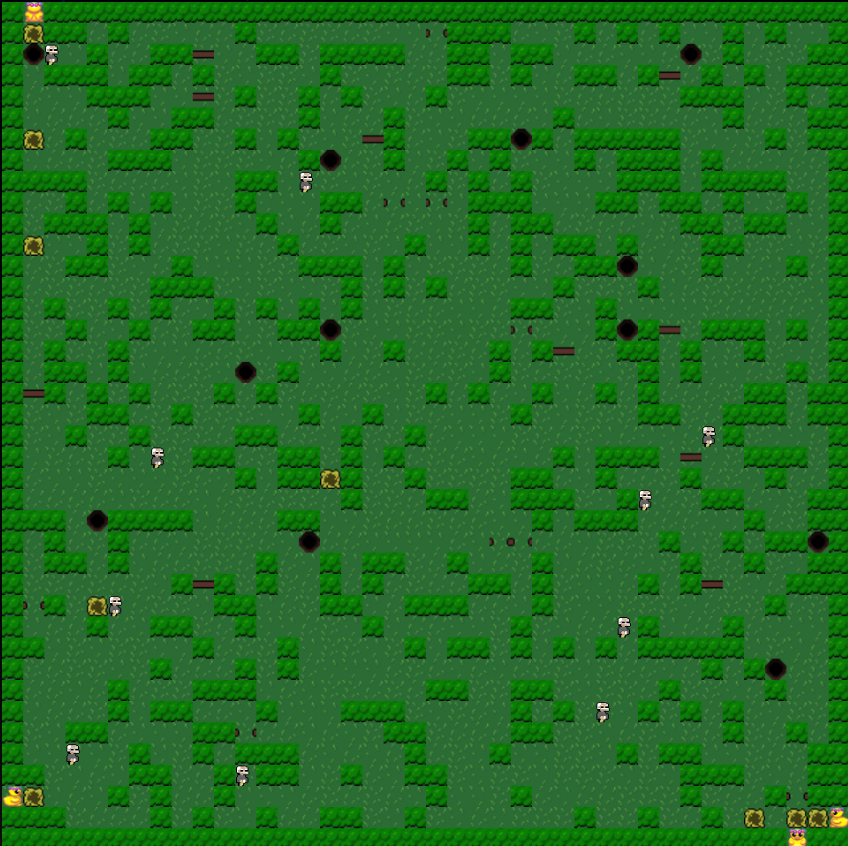
\includegraphics[width=0.7\textwidth]{img/map} 
    \end{center}
    \caption{Un parc}
    \label{fig:parc}
\end{figure}

%% Structure des cases :
% Représentation sur l'UI - Pour l'instant c'est un exemple, à remplacer
% Propriétés (constructibilité, traversabilité, mutabilité, ...)
% Spécificités

\subsection{Niveau Principal}

Le niveau principal correspond au niveau 0.
Il constitue le terrain essentiel du jeu.
Il est constitué dès l'initialisation de divers obstacles, et c'est sur ce terrain
uniquement qu'il est possible de gagner du score.
C'est sur ce niveau que sont situés les 4 points d'apparition.
Voici la liste exhaustive des différents types de cases qu'il est possible de
rencontrer au niveau principal :

\subsubsection{Gazon} 

Une case de type \texttt{GAZON} est représentée par du gazon.
%
Le gazon peut être constructible ou non, et cela est immuable tant que
personne ne construit sur la case.
Si une case de gazon est constructible, alors un joueur a la possibilité de poser un
buisson sur la case, ce qui change le type de la case en \texttt{BUISSON},
la rendant non traversable.
Le gazon est toujours traversable par une troupe.
%

\subsubsection{Buisson} 

Une case de type \texttt{BUISSON} est représentée par un buisson.
%
Un buisson n'est pas traversable ni constructible.
Un buisson est totalement immuable.

\subsubsection{Barrière}
\label{sec:barriere}

Une case de type \texttt{BARRIERE} est représentée par une barrière en bois,
ouverte ou fermée.
%
Une barrière ouverte est traversable, une barrière fermée n'est pas traversable.
Une barrière n'est pas constructible.
%
Au tour \texttt{TOUR\_FERMETURE} et uniquement à celui-ci, toute barrière fermée s'ouvre,
et toute barrière ouverte se ferme.
Une barrière se fermant au milieu d'une troupe entraîne la dispersion de la partie 
arrière de la troupe, du canard qui était présent sur le portique au vilain petit canard.
La partie avant de la troupe se disperse également si sa taille se retrouve
inférieure à \texttt{TAILLE\_MIN}.

\subsubsection{Nid}

Une case de type \texttt{NID} est représentée par un nid.
%
Un nid est toujours traversable et non constructible.
%
Chaque nid peut appartenir à un unique joueur ou à aucun des deux joueurs.
Un joueur peut prendre possession d'un nid n'appartenant encore à aucun joueur en
passant simplement l'une de ses mamans canards sur la case.
La prise d'un nid est automatique et ne nécessite aucune autre action.
Si une maman canard passe sur un nid lui appartenant, l'inventaire de la troupe
est vidé et le score est comptabilisé.
Rien ne se passe si une maman canard passe sur un nid adverse.

\subsubsection{Papy}

Une case de type \texttt{PAPY} est représentée par un papy\footnote{Il n'existe aucune interaction entre les cases de type \texttt{PAPY} et les pigeons contrairement à certains préjugés}.
%
Un papy est toujours traversable et non constructible.
%
De manière périodique, tous les \texttt{INTERVALLE\_DISTRIB} tours, chaque papy
dépose une miche de pain à ses pieds.
Cependant, tous les papys ne déposent pas une miche de pain en même temps.
Chaque papy possède une phase, c'est-à-dire le numéro du premier tour auquel le
papy va poser une miche de pain.
La phase peut être différente selon les papys. Un papy peut commencer à
distribuer une miche au 2$^{\text{ème}}$ tour puis tous les \texttt{INTERVALLE\_DISTRIB} tours,
tandis qu'un autre papy peut commencer à distribuer une miche au 3$^{\text{ème}}$ tour puis
tous les \texttt{INTERVALLE\_DISTRIB} tours.

\subsubsection{Trou}

Une case de type \texttt{TROU} est représentée par une fissure dans le sol.
% FIXME C'est faux, remplacer quand ce sera décidé
%
Un trou est toujours traversable et non constructible.
%
Si une maman canard se situe sur un trou, elle a la possibilité d'avancer vers
le bas afin d'accéder au niveau souterrain.
De la même manière, si une maman canard se situe sous un trou, elle a la
possibilité d'avancer vers le haut afin d'accéder au niveau principal. 

\subsection{Niveau Souterrain}

Le niveau souterrain correspond au niveau -1.
Le niveau souterrain est un niveau alternatif, initialement entièrement rempli de terre.
Contrairement au niveau principal, les joueurs peuvent \og creuser\fg{} ce niveau afin
de créer des raccourcis entre différents points du niveau principal.

\subsubsection{Terre}

Une case de type \texttt{TERRE} est représentée par un bloc de terre.
%
Un bloc de terre n'est ni traversable ni constructible.
En revanche, il est possible de creuser un bloc de terre \texttt{FREQ\_TUNNEL} fois
par tour, ce qui entraîne la transformation de ce bloc en un bloc de type
\texttt{TUNNEL}.
%

\subsubsection{Tunnel}

Une case de type \texttt{TUNNEL} est représentée par l'absence d'un bloc de terre\footnote{Vous ne pouvez creuser trop profond, pour ne pas déranger les nains standard !}.
%
Un tunnel est traversable mais pas constructible. Rien ne peut remplacer un tunnel.
%
Il est possible de remonter à la surface depuis un tunnel situé sous un trou en avançant vers le haut. 

\subsection{Format de la carte}

La carte du parc est représentée dans un fichier texte qui contient \texttt{HAUTEUR} lignes et \texttt{LARGEUR} caractères. Pour chaque caractères la représentation ASCII est :
\begin{center}
    \begin{tabular}{l|c|l}
        \hline
        \textbf{Type} & \textbf{Échantillon} & \textbf{Représentation} \\
        \hline
        Gazon non constructible & 
\includegraphics[width=.5cm]{img/sprite/grass.png} & \texttt{' '} (un espace) \\
        Gazon & 
\includegraphics[width=.5cm]{img/sprite/grass.png} & \texttt{'.'} \\
        Point d’apparition & 
\includegraphics[width=.5cm]{img/sprite/spawn.png} & \texttt{'S'} \\
        Buisson & 
\includegraphics[width=.5cm]{img/sprite/buisson.png} & \texttt{'\#'} \\
        Barrière ouverte & 
\includegraphics[width=.5cm]{img/sprite/gate.png} & \texttt{'B'} \\
        Barrière fermée & 
\includegraphics[width=.5cm]{img/sprite/gate_close.png} & \texttt{'b'} \\
        Nid & 
\includegraphics[width=.5cm]{img/sprite/nest_empty.png} & \texttt{'N'} \\
        Papy & 
\includegraphics[width=.5cm]{img/sprite/papy.png} & entre \texttt{'0'} et \texttt{'9'} \\
        Trou & 
\includegraphics[width=.5cm]{img/sprite/trou.png} & \texttt{'X'} \\
        \hline
    \end{tabular}
\end{center}

\section{Règles} 

\subsection{Début d'une partie}


Aucune miche de pain n'est présente sur la carte lors de l'initialisation de 
la partie.
Chaque joueur commence avec \texttt{NB\_TROUPES} troupes d'une taille de
\texttt{TAILLE\_DEPART}, situées sur des points d'apparition distincts.

\subsection{Apparition et dispersion}

Chaque carte dispose de 4 points d'apparition. Un point d'apparition est
situé sur chacune des bordures (Nord, Sud, Est, Ouest) de la carte.


% Besoin de préciser ? C'est l'initialisation, c'est pas important en soit
% vu qu'ils peuvent voir où sont leur troupes...
% Rep: Oui, ça peut être intéressant de savoir pour prédire les états futurs
%      (et aussi comprendre ce qu'il se passe)

% FIXME Cete partie (en dessous) n'aurai pas + sa place dans le déroulé d'un tour ?
% Rep: La partie a été renommée

Si un déplacement aurait impliqué que la maman canard se retrouve sur une case non
traversable ou sur la même case qu'un autre canard (d'une de vos troupes ou non),
cela entraîne une dispersion de l'entièreté de la troupe. La troupe qui a effectué le
mouvement, \textbf{et uniquement celle-ci}, se retire de la carte jusqu'à la fin du tour.
Au début du prochain tour, la troupe réapparaît, si possible,
au point d'apparition associé à la direction correspondant au mouvement tenté.
\footnote{Si une troupe tente d'aller vers le Nord alors qu'un mur se situe juste au Nord de sa
maman canard, alors la troupe se disperse, et tente de revenir au tour suivant depuis le
point d'apparition situé au Nord de la carte.}
Ainsi, les collisions entraînées par un mouvement vers le haut sont associées au point
d'apparition Nord, et les collisions entraînées par un mouvement vers le bas sont
associées au point d'apparition Sud.

Si le point d'apparition est déjà occupé par une troupe, alors le point d'apparition
choisi sera celui situé juste après celui prévu dans le sens horaire.

Lorsqu'une troupe apparaît, tous les canards n'apparaissent pas en même temps. Ils apparaissent en
effet, au fur et à mesure que la troupe avance. Ainsi, la taille de la troupe
augmente, commençant à 1 au moment de son apparition jusqu'à atteindre sa taille maximale lorsque
tous les canards sont présents.

\subsection{Déroulement d'un tour}

Chaque troupe possède \texttt{PTS\_ACTIONS} points d'action au début de son tour.
Tant qu'une troupe est sur le terrain et possède suffisamment de points d'action, elle peut, durant le même tour :

\begin{itemize}
    \item Avancer dans une direction, contre 1 de ses points d'action
    \item Grandir, contre \texttt{COUT\_CROISSANCE} de ses points d'action
\end{itemize}

De plus un joueur peut, \texttt{FREQ\_TUNNEL} fois durant un tour, et cela gratuitement,
creuser un bloc de terre du niveau souterrain.

Finalement, un joueur peut, à volonté, placer un buisson sur une case constructible,
en échange de \texttt{COUT\_BUISSON} points de score. Attention, ce coût est directement
prélevé du score, et il est nécessaire d'avoir un score suffisant pour placer le
buisson.

\textbf{Un tour ne peut se terminer que lorsqu'un joueur n'a plus de point d'action sur aucune de ses troupes ou plus de troupe disponible.}
Si un joueur termine son tour alors qu'une de ses troupes est encore sur le terrain
et possède toujours des points
d'action, cette troupe avancera automatiquement dans sa direction actuelle jusqu'à épuisement de ses points
d'action.

À la fin de chaque tour, les papys qui doivent déposer une miche de pain le font.

% Que tous les canards d'une roupe ne sont pas forcément display sur la map au spawn (vu que ça avance petit à petit)  ?
% Faire un point sur les possibilité de dispertio d'une troupe -> mur, canard, "plafond", "sol"

\subsection{Comptabilisation du score}

Lorsqu'une maman canard arrive sur un nid lui appartenant, l'inventaire de la troupe
est vidé sur le nid. Le score du joueur auquel la troupe appartient est augmenté en fonction
du nombre de miches de pain déposé. L'incrément de score est calculé par la fonction \texttt{gain}.
Globalement, sachez que, pour un nombre de miches de pain donné,
\textbf{il est bien plus intéressant tout déposer d'un seul coup plutôt qu'en plusieurs fois}.

% Fonction à déterminer

\section{Tournois}

\subsection{Tournois intermédiaires}

Afin de vous aider à perfectionner vos algorithmes, des tournois intermédiaires
vous seront proposés. Ces matchs n’ont absolument aucune influence sur le
classement final, mais sont néanmoins à prendre au sérieux, car ils vous
permettront de vous situer par rapport aux autres joueurs, de connaître vos
ennemis, vos points forts et vos faiblesses, et vous donneront des pistes pour
vous améliorer pendant la finale. L’annonce des tournois intermédiaires se fera
dans l’heure qui précède.

Pour chaque tournoi, nous prendrons le dernier
champion que chaque candidat aura envoyé sur le site de soumission pour le
faire participer au tournoi, et nous vous donnerons les résultats ainsi que
votre progression dès que les tournois se seront terminés, avec un
récapitulatif de votre progression globale. Les tournois seront exécutés sur
des cartes officielles de notre choix, qui seront potentiellement amenées à
changer au fur et à mesure.

Des tournois intermédiaires auront lieu\footnote{Nous nous réservons le droit de changer les horaires et le nombre de tournois intermédiaires} :
\begin{itemize}
    \item Vendredi 15 h 42 (tournoi test)
    \item Vendredi 17 h 42
    \item Vendredi 23 h 42
    \item Samedi 5 h 42
    \item Samedi 11 h 42
    \item Samedi 17 h 42
\end{itemize}

\subsection{Rendu final}

Le tournoi final aura lieu samedi à 23 h 42.

Le rendu final est le seul rendu qui comptera pour le classement. Les
mêmes règles s’appliquent : le dernier champion soumis à l’heure du début
du tournoi sera le champion utilisé pour le tournoi final.

Lors du tournoi final, plusieurs cartes seront ajoutées. Celles-ci resteront
inconnues de tous les joueurs jusqu’à la fin du concours, afin de mesurer
l’adaptabilité de vos algorithmes à des situations inconnues.

Pour le rendu final, nous vous demandons de rajouter des commentaires
qui résument le fonctionnement des différents blocs logiques de votre code,
ainsi qu'un \textbf{commentaire global en haut de votre fichier principal} qui détaille
votre stratégie ainsi que les différents algorithmes que vous avez employés
pour l’implémenter.

\section{Considérations techniques}

Vous disposez d’une seconde (temps réel !) à chaque fois qu'une de vos
fonctions est appelée pour rendre la main. Passé ce délai, votre programme est
tué, le match continue sans vous et vos fonctions ne sont plus appelées. Il n’est
pas possible de revenir en jeu tout simplement parce qu'il n’y a aucun moyen
de rétablir l’état des environnements des langages après une interruption. Les
limites de mémoire sont faites avec des cgroups, ce qui fait que l’allocation
échouera si vous essayez de dépasser la limite qui vous est accordée. Cette
limite compte aussi la taille de la pile.

D’autres limitations sont appliquées :
\begin{itemize}
    \item le système de fichiers est entièrement en lecture seule ;
    \item seuls /usr, /var et /tmp sont montés ;
    \item vous n’avez pas le droit d’utiliser des processus en parallèle ;
    \item la mémoire est limitée à 500 Mio ;
    \item la taille totale de votre output ne doit pas dépasser 256 Kio (elle sera tronquée à partir de cette limite) ;
    \item le temps d’exécution total du processus est limité à 300 secondes de temps réel ;
    \item chaque appel de fonction est limité à une seconde de temps réel plus
500 millisecondes de marge pour prendre en compte le surcoût de sérialisation/désérialisation des valeurs depuis et vers les langages cibles.
\end{itemize}


\newpage

\newpage
\section{API}
% This file was generated by stechec2-generator. DO NOT EDIT.

\noindent \begin{tabular}{lp{11cm}}
\textbf{Constante:} & HAUTEUR \\
\textbf{Valeur:} & 40 \\
\textbf{Description:} & Nombre de lignes dans la carte \\
\end{tabular}
\vspace{0.2cm} \\

\noindent \begin{tabular}{lp{11cm}}
\textbf{Constante:} & LARGEUR \\
\textbf{Valeur:} & 40 \\
\textbf{Description:} & Nombre de colonnes dans la carte \\
\end{tabular}
\vspace{0.2cm} \\

\noindent \begin{tabular}{lp{11cm}}
\textbf{Constante:} & NB\_TOURS \\
\textbf{Valeur:} & 400 \\
\textbf{Description:} & Nombre de tours à jouer avant la fin de la partie \\
\end{tabular}
\vspace{0.2cm} \\

\noindent \begin{tabular}{lp{11cm}}
\textbf{Constante:} & TAILLE\_DEPART \\
\textbf{Valeur:} & 5 \\
\textbf{Description:} & Taille de départ d'une troupe \\
\end{tabular}
\vspace{0.2cm} \\

\noindent \begin{tabular}{lp{11cm}}
\textbf{Constante:} & TAILLE\_MIN \\
\textbf{Valeur:} & 3 \\
\textbf{Description:} & Taille minimale qu'une troupe peut avoir avant de se disperser \\
\end{tabular}
\vspace{0.2cm} \\

\noindent \begin{tabular}{lp{11cm}}
\textbf{Constante:} & NB\_TROUPES \\
\textbf{Valeur:} & 2 \\
\textbf{Description:} & Nombre de troupes que chaque joueur controle \\
\end{tabular}
\vspace{0.2cm} \\

\noindent \begin{tabular}{lp{11cm}}
\textbf{Constante:} & INTERVALLE\_DISTRIB \\
\textbf{Valeur:} & 5 \\
\textbf{Description:} & Intervalle de distribution de pains par les papys \\
\end{tabular}
\vspace{0.2cm} \\

\noindent \begin{tabular}{lp{11cm}}
\textbf{Constante:} & FREQ\_TUNNEL \\
\textbf{Valeur:} & 1 \\
\textbf{Description:} & Nombre de tunnels qu'un joueur peut creuser par tour \\
\end{tabular}
\vspace{0.2cm} \\

\noindent \begin{tabular}{lp{11cm}}
\textbf{Constante:} & PTS\_ACTION \\
\textbf{Valeur:} & 5 \\
\textbf{Description:} & Nombre de déplacements que peut faire une troupe en un tour \\
\end{tabular}
\vspace{0.2cm} \\

\noindent \begin{tabular}{lp{11cm}}
\textbf{Constante:} & COUT\_CROISSANCE \\
\textbf{Valeur:} & 3 \\
\textbf{Description:} & Nombre de points de mouvement requis pour incrémenter la taille \\
\end{tabular}
\vspace{0.2cm} \\

\noindent \begin{tabular}{lp{11cm}}
\textbf{Constante:} & COUT\_BUISSON \\
\textbf{Valeur:} & 3 \\
\textbf{Description:} & Coût en score de la pose de buisson \\
\end{tabular}
\vspace{0.2cm} \\

\noindent \begin{tabular}{lp{11cm}}
\textbf{Constante:} & ROUND\_FERMETURE \\
\textbf{Valeur:} & 99 \\
\textbf{Description:} & Round à la fin duquel les barrières s'ouvrent ou se ferment \\
\end{tabular}
\vspace{0.2cm} \\


\functitle{erreur} \\
\noindent
\begin{tabular}[t]{@{\extracolsep{0pt}}>{\bfseries}lp{10cm}}
Description~: & Erreurs possibles après avoir effectué une action \\
Valeurs~: &
\small
\begin{tabular}[t]{@{\extracolsep{0pt}}lp{7cm}}
    \textsl{OK}~: & L'action a été effectuée avec succès \\
    \textsl{TROUPE\_INVALIDE}~: & Mauvais identifiant de troupe \\
    \textsl{HORS\_TOUR}~: & Aucune action n'est possible hors de joueur\_tour \\
    \textsl{MOUVEMENTS\_INSUFFISANTS}~: & Il ne reste plus assez de points de mouvements pour effectuer l'action demandée \\
    \textsl{TROP\_GRANDI}~: & La troupe a déjà trop grandi pendant le tour \\
    \textsl{TROP\_CREUSE}~: & Trop de trous ont déjà été creusés pendant le tour \\
    \textsl{NON\_CREUSABLE}~: & Il n'est pas possible de creuser à la position demandée \\
    \textsl{NON\_CONSTRUCTIBLE}~: & La zone demandée n'est pas constructible \\
    \textsl{SCORE\_INSUFFISANT}~: & Le joueur n'a pas assez de points pour construire un buisson \\
    \textsl{POSITION\_INVALIDE}~: & La position demandée est hors du parc \\
    \textsl{DIRECTION\_INVALIDE}~: & La direction spécifiée n'existe pas. \\
    \textsl{PIGEON\_INVALIDE}~: & Le pigeon spécifié n'existe pas. \\
\end{tabular} \\
\end{tabular}

\functitle{direction} \\
\noindent
\begin{tabular}[t]{@{\extracolsep{0pt}}>{\bfseries}lp{10cm}}
Description~: & Directions possibles \\
Valeurs~: &
\small
\begin{tabular}[t]{@{\extracolsep{0pt}}lp{7cm}}
    \textsl{NORD}~: & Sens positif pour les lignes \\
    \textsl{SUD}~: & Sens négatif pour les lignes \\
    \textsl{EST}~: & Sens positif pour les colonnes \\
    \textsl{OUEST}~: & Sens négatif pour les colonnes \\
    \textsl{HAUT}~: & Sens positif pour le niveau \\
    \textsl{BAS}~: & Sens négatif pour le niveau \\
\end{tabular} \\
\end{tabular}

\functitle{type\_case} \\
\noindent
\begin{tabular}[t]{@{\extracolsep{0pt}}>{\bfseries}lp{10cm}}
Description~: & Type de l'élément présent sur une case \\
Valeurs~: &
\small
\begin{tabular}[t]{@{\extracolsep{0pt}}lp{7cm}}
    \textsl{GAZON}~: & Absence d'élément \\
    \textsl{BUISSON}~: & Obstacle impossible à traverser \\
    \textsl{BARRIERE}~: & Élément pouvant être ouvert ou fermé. Une barrière fermée est infranchissable alors qu'une barrière ouverte est analogue à une case vide \\
    \textsl{NID}~: & Élément traversable permettant à la troupe de déposer son inventaire en échange de points \\
    \textsl{PAPY}~: & Élément traversable générant de manière périodique des miches de pain \\
    \textsl{TROU}~: & Interface entre le niveau principal est le niveau souterrain \\
    \textsl{TUNNEL}~: & Bloc du souterrain ayant été creusé \\
    \textsl{TERRE}~: & Bloc du souterrain n'ayant pas encore été creusé \\
\end{tabular} \\
\end{tabular}

\functitle{etat\_barriere} \\
\noindent
\begin{tabular}[t]{@{\extracolsep{0pt}}>{\bfseries}lp{10cm}}
Description~: & État d'une barrière, soit ouvert, soit fermé, soit non-applicable \\
Valeurs~: &
\small
\begin{tabular}[t]{@{\extracolsep{0pt}}lp{7cm}}
    \textsl{OUVERTE}~: & La barrière est ouverte \\
    \textsl{FERMEE}~: & La barrière est fermée \\
    \textsl{PAS\_DE\_BARRIERE}~: & L'élément dont on requiert l'état n'est pas une barrière \\
\end{tabular} \\
\end{tabular}

\functitle{etat\_nid} \\
\noindent
\begin{tabular}[t]{@{\extracolsep{0pt}}>{\bfseries}lp{10cm}}
Description~: & Joueur auquel appartient un nid \\
Valeurs~: &
\small
\begin{tabular}[t]{@{\extracolsep{0pt}}lp{7cm}}
    \textsl{LIBRE}~: & Le nid n'a pas été attribué \\
    \textsl{JOUEUR\_0}~: & Joueur 0 \\
    \textsl{JOUEUR\_1}~: & Joueur 1 \\
    \textsl{PAS\_DE\_NID}~: & L'élément dont on requiert l'état n'est pas un nid \\
\end{tabular} \\
\end{tabular}

\functitle{pigeon\_debug} \\
\noindent
\begin{tabular}[t]{@{\extracolsep{0pt}}>{\bfseries}lp{10cm}}
Description~: & Type de pigeon de debug \\
Valeurs~: &
\small
\begin{tabular}[t]{@{\extracolsep{0pt}}lp{7cm}}
    \textsl{PAS\_DE\_PIGEON}~: & Aucun pigeon, enlève le pigeon présent \\
    \textsl{PIGEON\_BLEU}~: & Pigeon bleu \\
    \textsl{PIGEON\_JAUNE}~: & Pigeon jaune \\
    \textsl{PIGEON\_ROUGE}~: & Pigeon rouge \\
\end{tabular} \\
\end{tabular}

\functitle{type\_action} \\
\noindent
\begin{tabular}[t]{@{\extracolsep{0pt}}>{\bfseries}lp{10cm}}
Description~: & Types d'actions \\
Valeurs~: &
\small
\begin{tabular}[t]{@{\extracolsep{0pt}}lp{7cm}}
    \textsl{ACTION\_AVANCER}~: & Action ``avancer`` \\
    \textsl{ACTION\_GRANDIR}~: & Action ``grandir`` \\
    \textsl{ACTION\_CONSTRUIRE}~: & Action ``construire buisson`` \\
    \textsl{ACTION\_CREUSER}~: & Action ``creuser tunnel`` \\
\end{tabular} \\
\end{tabular}



\functitle{position}
\begin{lst-c++}
struct position {
    int colonne;
    int ligne;
    int niveau;
};
\end{lst-c++}
\noindent
\begin{tabular}[t]{@{\extracolsep{0pt}}>{\bfseries}lp{10cm}}
Description~: & Position dans la carte, donnée par trois coordonnées \\
Champs~: &
\small
\begin{tabular}[t]{@{\extracolsep{0pt}}lp{7cm}}
    \textsl{colonne}~: & Abscisse \\
    \textsl{ligne}~: & Ordonnée \\
    \textsl{niveau}~: & Niveau \\
\end{tabular} \\
\end{tabular}

\functitle{troupe}
\begin{lst-c++}
struct troupe {
    position maman;
    position array canards;
    int taille;
    direction dir;
    int inventaire;
    int pts\_action;
    int id;
};
\end{lst-c++}
\noindent
\begin{tabular}[t]{@{\extracolsep{0pt}}>{\bfseries}lp{10cm}}
Description~: & Une troupe, composée de la maman canard et de ses canetons \\
Champs~: &
\small
\begin{tabular}[t]{@{\extracolsep{0pt}}lp{7cm}}
    \textsl{maman}~: & Position de la maman canard \\
    \textsl{canards}~: & Position des différents canards de la troupe, incluant la maman en première position \\
    \textsl{taille}~: & Taille de la troupe \\
    \textsl{dir}~: & Direction de la troupe \\
    \textsl{inventaire}~: & Nombre de pains de la troupe \\
    \textsl{pts\_action}~: & Nombre de points d'action de la troupe \\
    \textsl{id}~: & Identifiant de la troupe \\
\end{tabular} \\
\end{tabular}

\functitle{etat\_case}
\begin{lst-c++}
struct etat\_case {
    position pos;
    type\_case contenu;
    bool est\_constructible;
    int nb\_pains;
};
\end{lst-c++}
\noindent
\begin{tabular}[t]{@{\extracolsep{0pt}}>{\bfseries}lp{10cm}}
Description~: & Élément constituant le parc \\
Champs~: &
\small
\begin{tabular}[t]{@{\extracolsep{0pt}}lp{7cm}}
    \textsl{pos}~: & Position de la case. Le niveau vaut nécessairement 0 \\
    \textsl{contenu}~: & Type de la case \\
    \textsl{est\_constructible}~: & La case est constructible \\
    \textsl{nb\_pains}~: & Nombre de pains contenus sur la case \\
\end{tabular} \\
\end{tabular}

\functitle{action\_hist}
\begin{lst-c++}
struct action\_hist {
    type\_action action\_type;
    int troupe\_id;
    direction action\_dir;
    position action\_pos;
};
\end{lst-c++}
\noindent
\begin{tabular}[t]{@{\extracolsep{0pt}}>{\bfseries}lp{10cm}}
Description~: & Action représentée dans l'historique \\
Champs~: &
\small
\begin{tabular}[t]{@{\extracolsep{0pt}}lp{7cm}}
    \textsl{action\_type}~: & Type de l'action \\
    \textsl{troupe\_id}~: & Identifiant de la troupe \\
    \textsl{action\_dir}~: & Direction de l'action \\
    \textsl{action\_pos}~: & Position de l'action \\
\end{tabular} \\
\end{tabular}



\begin{minipage}{\linewidth}
\functitle{avancer}
\begin{lst-c++}
erreur avancer(int id, direction dir)
\end{lst-c++}
\noindent
\begin{tabular}[t]{@{\extracolsep{0pt}}>{\bfseries}lp{10cm}}
Description~: & La troupe avance d'une case vers une direction donnée \\
Paramètres~: &
\begin{tabular}[t]{@{\extracolsep{0pt}}ll}
    \textsl{id}~: & Identifiant de la troupe à avancer \\
    \textsl{dir}~: & Direction vers laquelle avancer \\
  \end{tabular} \\
\end{tabular} \\[0.3cm]
\end{minipage}

\begin{minipage}{\linewidth}
\functitle{grandir}
\begin{lst-c++}
erreur grandir(int id)
\end{lst-c++}
\noindent
\begin{tabular}[t]{@{\extracolsep{0pt}}>{\bfseries}lp{10cm}}
Description~: & La troupe grandit \\
Paramètres~: &
\begin{tabular}[t]{@{\extracolsep{0pt}}ll}
    \textsl{id}~: & Identifiant de la troupe à faire grandir \\
  \end{tabular} \\
\end{tabular} \\[0.3cm]
\end{minipage}

\begin{minipage}{\linewidth}
\functitle{construire\_buisson}
\begin{lst-c++}
erreur construire\_buisson(position pos)
\end{lst-c++}
\noindent
\begin{tabular}[t]{@{\extracolsep{0pt}}>{\bfseries}lp{10cm}}
Description~: & Construit un buisson à la position donnée \\
Paramètres~: &
\begin{tabular}[t]{@{\extracolsep{0pt}}ll}
    \textsl{pos}~: & Position où construire le buisson \\
  \end{tabular} \\
\end{tabular} \\[0.3cm]
\end{minipage}

\begin{minipage}{\linewidth}
\functitle{creuser\_tunnel}
\begin{lst-c++}
erreur creuser\_tunnel(position pos)
\end{lst-c++}
\noindent
\begin{tabular}[t]{@{\extracolsep{0pt}}>{\bfseries}lp{10cm}}
Description~: & Creuse un tunnel à la position donnée \\
Paramètres~: &
\begin{tabular}[t]{@{\extracolsep{0pt}}ll}
    \textsl{pos}~: & Position de la case à creuser \\
  \end{tabular} \\
\end{tabular} \\[0.3cm]
\end{minipage}

\begin{minipage}{\linewidth}
\functitle{info\_case}
\begin{lst-c++}
etat\_case info\_case(position pos)
\end{lst-c++}
\noindent
\begin{tabular}[t]{@{\extracolsep{0pt}}>{\bfseries}lp{10cm}}
Description~: & Renvoie les informations concernant une case \\
Paramètres~: &
\begin{tabular}[t]{@{\extracolsep{0pt}}ll}
    \textsl{pos}~: & Position de la case \\
  \end{tabular} \\
\end{tabular} \\[0.3cm]
\end{minipage}

\begin{minipage}{\linewidth}
\functitle{info\_barriere}
\begin{lst-c++}
etat\_barriere info\_barriere(position pos)
\end{lst-c++}
\noindent
\begin{tabular}[t]{@{\extracolsep{0pt}}>{\bfseries}lp{10cm}}
Description~: & Renvoie les informations d'état d'une barrière \\
Paramètres~: &
\begin{tabular}[t]{@{\extracolsep{0pt}}ll}
    \textsl{pos}~: & Position de la barrière \\
  \end{tabular} \\
\end{tabular} \\[0.3cm]
\end{minipage}

\begin{minipage}{\linewidth}
\functitle{info\_nid}
\begin{lst-c++}
etat\_nid info\_nid(position pos)
\end{lst-c++}
\noindent
\begin{tabular}[t]{@{\extracolsep{0pt}}>{\bfseries}lp{10cm}}
Description~: & Renvoie les informations d'état d'un nid \\
Paramètres~: &
\begin{tabular}[t]{@{\extracolsep{0pt}}ll}
    \textsl{pos}~: & Position du nid \\
  \end{tabular} \\
\end{tabular} \\[0.3cm]
\end{minipage}

\begin{minipage}{\linewidth}
\functitle{papy\_tours\_restants}
\begin{lst-c++}
int papy\_tours\_restants(position pos)
\end{lst-c++}
\noindent
\begin{tabular}[t]{@{\extracolsep{0pt}}>{\bfseries}lp{10cm}}
Description~: & Renvoie le nombre de tours restants avant qu'un papy dépose une miche de pain. Retourne -1 si aucun papy ne se trouve à la position demandée \\
Paramètres~: &
\begin{tabular}[t]{@{\extracolsep{0pt}}ll}
    \textsl{pos}~: & Position du papy \\
  \end{tabular} \\
\end{tabular} \\[0.3cm]
\end{minipage}

\begin{minipage}{\linewidth}
\functitle{troupes\_joueur}
\begin{lst-c++}
troupe array troupes\_joueur(int id\_joueur)
\end{lst-c++}
\noindent
\begin{tabular}[t]{@{\extracolsep{0pt}}>{\bfseries}lp{10cm}}
Description~: & Renvoie les troupes d'un joueur. Si le joueur est invalide, tous les champs valent -1. \\
Paramètres~: &
\begin{tabular}[t]{@{\extracolsep{0pt}}ll}
    \textsl{id\_joueur}~: & Numéro du joueur concerné \\
  \end{tabular} \\
\end{tabular} \\[0.3cm]
\end{minipage}

\begin{minipage}{\linewidth}
\functitle{pains}
\begin{lst-c++}
position array pains()
\end{lst-c++}
\noindent
\begin{tabular}[t]{@{\extracolsep{0pt}}>{\bfseries}lp{10cm}}
Description~: & Renvoie la position des pains récupérables \\
\end{tabular} \\[0.3cm]
\end{minipage}

\begin{minipage}{\linewidth}
\functitle{debug\_poser\_pigeon}
\begin{lst-c++}
erreur debug\_poser\_pigeon(position pos, pigeon\_debug pigeon)
\end{lst-c++}
\noindent
\begin{tabular}[t]{@{\extracolsep{0pt}}>{\bfseries}lp{10cm}}
Description~: & Pose un pigeon de debug sur la case indiquée \\
Paramètres~: &
\begin{tabular}[t]{@{\extracolsep{0pt}}ll}
    \textsl{pos}~: & Case où poser le pigeon \\
    \textsl{pigeon}~: & Pigeon à afficher sur la case \\
  \end{tabular} \\
\end{tabular} \\[0.3cm]
\end{minipage}

\begin{minipage}{\linewidth}
\functitle{historique}
\begin{lst-c++}
action\_hist array historique()
\end{lst-c++}
\noindent
\begin{tabular}[t]{@{\extracolsep{0pt}}>{\bfseries}lp{10cm}}
Description~: & Renvoie la liste des actions effectuées par l'adversaire durant son tour, dans l'ordre chronologique. Les actions de débug n'apparaissent pas dans cette liste. \\
\end{tabular} \\[0.3cm]
\end{minipage}

\begin{minipage}{\linewidth}
\functitle{gain}
\begin{lst-c++}
int gain(int nb\_pains)
\end{lst-c++}
\noindent
\begin{tabular}[t]{@{\extracolsep{0pt}}>{\bfseries}lp{10cm}}
Description~: & Renvoie le gain en score que le nombre de pains passé en entrée rapporterait s'ils étaient tous déposés d'un coup dans un nid \\
Paramètres~: &
\begin{tabular}[t]{@{\extracolsep{0pt}}ll}
    \textsl{nb\_pains}~: & Nombre de miches de pain déposées \\
  \end{tabular} \\
\end{tabular} \\[0.3cm]
\end{minipage}

\begin{minipage}{\linewidth}
\functitle{inventaire}
\begin{lst-c++}
int inventaire(int taille)
\end{lst-c++}
\noindent
\begin{tabular}[t]{@{\extracolsep{0pt}}>{\bfseries}lp{10cm}}
Description~: & Renvoie la taille de l'inventaire d'une troupe de taille donnée \\
Paramètres~: &
\begin{tabular}[t]{@{\extracolsep{0pt}}ll}
    \textsl{taille}~: & Taille de la troupe \\
  \end{tabular} \\
\end{tabular} \\[0.3cm]
\end{minipage}

\begin{minipage}{\linewidth}
\functitle{trouver\_chemin}
\begin{lst-c++}
direction array trouver\_chemin(position depart, position arrivee)
\end{lst-c++}
\noindent
\begin{tabular}[t]{@{\extracolsep{0pt}}>{\bfseries}lp{10cm}}
Description~: & Trouve un plus court chemin ouvert entre deux positions. Renvoie une liste vide si les deux positions sont égales ou si aucun chemin n'existe. \\
Paramètres~: &
\begin{tabular}[t]{@{\extracolsep{0pt}}ll}
    \textsl{depart}~: & Position de départ \\
    \textsl{arrivee}~: & Position d'arrivée \\
  \end{tabular} \\
\end{tabular} \\[0.3cm]
\end{minipage}

\begin{minipage}{\linewidth}
\functitle{moi}
\begin{lst-c++}
int moi()
\end{lst-c++}
\noindent
\begin{tabular}[t]{@{\extracolsep{0pt}}>{\bfseries}lp{10cm}}
Description~: & Renvoie votre numéro de joueur. \\
\end{tabular} \\[0.3cm]
\end{minipage}

\begin{minipage}{\linewidth}
\functitle{adversaire}
\begin{lst-c++}
int adversaire()
\end{lst-c++}
\noindent
\begin{tabular}[t]{@{\extracolsep{0pt}}>{\bfseries}lp{10cm}}
Description~: & Renvoie le numéro du joueur adverse. \\
\end{tabular} \\[0.3cm]
\end{minipage}

\begin{minipage}{\linewidth}
\functitle{score}
\begin{lst-c++}
int score(int id\_joueur)
\end{lst-c++}
\noindent
\begin{tabular}[t]{@{\extracolsep{0pt}}>{\bfseries}lp{10cm}}
Description~: & Renvoie le score du joueur `id\_joueur`. Renvoie -1 si le joueur est invalide. \\
Paramètres~: &
\begin{tabular}[t]{@{\extracolsep{0pt}}ll}
    \textsl{id\_joueur}~: & Numéro du joueur concerné \\
  \end{tabular} \\
\end{tabular} \\[0.3cm]
\end{minipage}

\begin{minipage}{\linewidth}
\functitle{annuler}
\begin{lst-c++}
bool annuler()
\end{lst-c++}
\noindent
\begin{tabular}[t]{@{\extracolsep{0pt}}>{\bfseries}lp{10cm}}
Description~: & Annule la dernière action. Renvoie faux quand il n'y a pas d'action à annuler ce tour-ci \\
\end{tabular} \\[0.3cm]
\end{minipage}

\begin{minipage}{\linewidth}
\functitle{tour\_actuel}
\begin{lst-c++}
int tour\_actuel()
\end{lst-c++}
\noindent
\begin{tabular}[t]{@{\extracolsep{0pt}}>{\bfseries}lp{10cm}}
Description~: & Retourne le numéro du tour actuel. \\
\end{tabular} \\[0.3cm]
\end{minipage}

\begin{minipage}{\linewidth}
\functitle{afficher\_erreur}
\begin{lst-c++}
void afficher\_erreur(erreur v)
\end{lst-c++}
\noindent
\begin{tabular}[t]{@{\extracolsep{0pt}}>{\bfseries}lp{10cm}}
Description~: & Affiche le contenu d'une valeur de type erreur \\
Paramètres~: &
\begin{tabular}[t]{@{\extracolsep{0pt}}ll}
    \textsl{v}~: & The value to display \\
  \end{tabular} \\
\end{tabular} \\[0.3cm]
\end{minipage}

\begin{minipage}{\linewidth}
\functitle{afficher\_direction}
\begin{lst-c++}
void afficher\_direction(direction v)
\end{lst-c++}
\noindent
\begin{tabular}[t]{@{\extracolsep{0pt}}>{\bfseries}lp{10cm}}
Description~: & Affiche le contenu d'une valeur de type direction \\
Paramètres~: &
\begin{tabular}[t]{@{\extracolsep{0pt}}ll}
    \textsl{v}~: & The value to display \\
  \end{tabular} \\
\end{tabular} \\[0.3cm]
\end{minipage}

\begin{minipage}{\linewidth}
\functitle{afficher\_type\_case}
\begin{lst-c++}
void afficher\_type\_case(type\_case v)
\end{lst-c++}
\noindent
\begin{tabular}[t]{@{\extracolsep{0pt}}>{\bfseries}lp{10cm}}
Description~: & Affiche le contenu d'une valeur de type type\_case \\
Paramètres~: &
\begin{tabular}[t]{@{\extracolsep{0pt}}ll}
    \textsl{v}~: & The value to display \\
  \end{tabular} \\
\end{tabular} \\[0.3cm]
\end{minipage}

\begin{minipage}{\linewidth}
\functitle{afficher\_etat\_barriere}
\begin{lst-c++}
void afficher\_etat\_barriere(etat\_barriere v)
\end{lst-c++}
\noindent
\begin{tabular}[t]{@{\extracolsep{0pt}}>{\bfseries}lp{10cm}}
Description~: & Affiche le contenu d'une valeur de type etat\_barriere \\
Paramètres~: &
\begin{tabular}[t]{@{\extracolsep{0pt}}ll}
    \textsl{v}~: & The value to display \\
  \end{tabular} \\
\end{tabular} \\[0.3cm]
\end{minipage}

\begin{minipage}{\linewidth}
\functitle{afficher\_etat\_nid}
\begin{lst-c++}
void afficher\_etat\_nid(etat\_nid v)
\end{lst-c++}
\noindent
\begin{tabular}[t]{@{\extracolsep{0pt}}>{\bfseries}lp{10cm}}
Description~: & Affiche le contenu d'une valeur de type etat\_nid \\
Paramètres~: &
\begin{tabular}[t]{@{\extracolsep{0pt}}ll}
    \textsl{v}~: & The value to display \\
  \end{tabular} \\
\end{tabular} \\[0.3cm]
\end{minipage}

\begin{minipage}{\linewidth}
\functitle{afficher\_pigeon\_debug}
\begin{lst-c++}
void afficher\_pigeon\_debug(pigeon\_debug v)
\end{lst-c++}
\noindent
\begin{tabular}[t]{@{\extracolsep{0pt}}>{\bfseries}lp{10cm}}
Description~: & Affiche le contenu d'une valeur de type pigeon\_debug \\
Paramètres~: &
\begin{tabular}[t]{@{\extracolsep{0pt}}ll}
    \textsl{v}~: & The value to display \\
  \end{tabular} \\
\end{tabular} \\[0.3cm]
\end{minipage}

\begin{minipage}{\linewidth}
\functitle{afficher\_type\_action}
\begin{lst-c++}
void afficher\_type\_action(type\_action v)
\end{lst-c++}
\noindent
\begin{tabular}[t]{@{\extracolsep{0pt}}>{\bfseries}lp{10cm}}
Description~: & Affiche le contenu d'une valeur de type type\_action \\
Paramètres~: &
\begin{tabular}[t]{@{\extracolsep{0pt}}ll}
    \textsl{v}~: & The value to display \\
  \end{tabular} \\
\end{tabular} \\[0.3cm]
\end{minipage}

\begin{minipage}{\linewidth}
\functitle{afficher\_position}
\begin{lst-c++}
void afficher\_position(position v)
\end{lst-c++}
\noindent
\begin{tabular}[t]{@{\extracolsep{0pt}}>{\bfseries}lp{10cm}}
Description~: & Affiche le contenu d'une valeur de type position \\
Paramètres~: &
\begin{tabular}[t]{@{\extracolsep{0pt}}ll}
    \textsl{v}~: & The value to display \\
  \end{tabular} \\
\end{tabular} \\[0.3cm]
\end{minipage}

\begin{minipage}{\linewidth}
\functitle{afficher\_troupe}
\begin{lst-c++}
void afficher\_troupe(troupe v)
\end{lst-c++}
\noindent
\begin{tabular}[t]{@{\extracolsep{0pt}}>{\bfseries}lp{10cm}}
Description~: & Affiche le contenu d'une valeur de type troupe \\
Paramètres~: &
\begin{tabular}[t]{@{\extracolsep{0pt}}ll}
    \textsl{v}~: & The value to display \\
  \end{tabular} \\
\end{tabular} \\[0.3cm]
\end{minipage}

\begin{minipage}{\linewidth}
\functitle{afficher\_etat\_case}
\begin{lst-c++}
void afficher\_etat\_case(etat\_case v)
\end{lst-c++}
\noindent
\begin{tabular}[t]{@{\extracolsep{0pt}}>{\bfseries}lp{10cm}}
Description~: & Affiche le contenu d'une valeur de type etat\_case \\
Paramètres~: &
\begin{tabular}[t]{@{\extracolsep{0pt}}ll}
    \textsl{v}~: & The value to display \\
  \end{tabular} \\
\end{tabular} \\[0.3cm]
\end{minipage}

\begin{minipage}{\linewidth}
\functitle{afficher\_action\_hist}
\begin{lst-c++}
void afficher\_action\_hist(action\_hist v)
\end{lst-c++}
\noindent
\begin{tabular}[t]{@{\extracolsep{0pt}}>{\bfseries}lp{10cm}}
Description~: & Affiche le contenu d'une valeur de type action\_hist \\
Paramètres~: &
\begin{tabular}[t]{@{\extracolsep{0pt}}ll}
    \textsl{v}~: & The value to display \\
  \end{tabular} \\
\end{tabular} \\[0.3cm]
\end{minipage}



\newpage
\section{Notes sur l'utilisation de l'API}
\subsection{C}

\begin{itemize}
\item{Les booléens sont représentés par le type \texttt{bool}, défini par le
      standard du C99, et que l'on retrouve dans le header \texttt{stdbool.h};}
\item{Les fonctions prenant des tableaux en paramètres et retournant des
      tableaux utilisent à la place de ces tableaux une structure
      \texttt{type\_array}, où \texttt{type} est le type des données dans le
      tableau. Ces structures contiennent deux éléments : les données,
      \texttt{type* items}, et la taille, \texttt{size\_t length}. Dans tous les
      cas, la libération des données est laissée au soin du candidat ;}
\item{Tout le reste est comme indiqué dans le sujet.}
\end{itemize}

\subsection{C++}

\begin{itemize}
\item{Les tableaux sont représentés par des \texttt{std::vector<type>} ;}
\item{Le reste est identique au sujet.}
\end{itemize}

\subsection{C\#}

\begin{itemize}
\item{Les fonctions à utiliser sont des méthodes statiques de la classe
      \texttt{Api}.
      Ainsi, pour utiliser la fonction \texttt{Foo}, il faut faire
      \texttt{Api.Foo} ;}
\item{Les noms des fonctions, structures et énumérations sont en
      \texttt{CamelCase}. Ainsi, une fonction nommée \texttt{foo\_bar} dans
      le sujet s'appellera \texttt{FooBar} en C\#.}
\end{itemize}

\subsection{Haskell}

\begin{itemize}
\item{L'API est fournie par le module \texttt{Api}.}
\item{Les énumérations sont représentées par des types sommes, les structures
      par des records. Seule la première lettre des noms de types et de
      constructeurs est en majuscule. Le nom du constructeur d'une structure
      est son nom de type.}
\item{La commande \texttt{make doc} permet de générer la documentation dans le
      fichier \texttt{doc/index.html} pour votre code ainsi que pour l'API.}
\item{Pour pouvoir conserver des valeurs entre différents appels à vos fonctions
      à compléter, il faut utiliser des variables mutables :}
\begin{lstlisting}[language=Haskell]
import Data.IORef
import System.IO.Unsafe (unsafePerformIO)

-- La pragma NOINLINE est importante !
-- MonType ne doit pas etre polymorphe !
{-# NOINLINE maVariable #-}
maVariable :: IORef MonType
maVariable = unsafePerformIO (newIORef maValeurInitiale)

fonctionACompleter :: IO ()
fonctionACompleter = do
  maValeur <- readIORef maVariable
  ...
  writeIORef maVariable maValeur'

\end{lstlisting}
\end{itemize}

\subsection{Java}

\begin{itemize}
\item{Les fonctions à utiliser sont des méthodes statiques de la classe
      \texttt{Interface}. Ainsi, pour utiliser la fonction \texttt{foo}, il
      faut faire \texttt{Interface.foo} ;}
\item{Les structures sont représentées par des classes dont tous les attributs
      sont publics.}
\end{itemize}

\subsection{OCaml}

\begin{itemize}
\item{L'API est fournie par le fichier \texttt{api.ml}, qui est \texttt{open}
      par défaut par le fichier à compléter ;}
\item{Les énumérations sont représentées par des types sommes avec des
      constructeurs sans paramètres. Seule la première lettre des noms des
      constructeurs est en majuscule ;}

\item{Les structures sont représentées par des records, sauf pour la structure
      \texttt{position} qui est représentée par un couple \texttt{int * int} ;}
\item{Les tableaux sont représentés par des \texttt{array} Caml classiques.}
\end{itemize}

\subsection{PHP}

\begin{itemize}
\item{Les constantes sont définies via des \texttt{define} et doivent donc être
      utilisées sans les précéder d'un signe dollar ;}
\item{Les énumérations sont définies comme des séries de constantes. Se référer
      à la puce au-dessus ;}
\item{Les structures sont gérées sous forme de tableaux associatifs. Ainsi, une
      structure contenant un champ \texttt{x} et un champ \texttt{y} sera créée
      comme ceci : \texttt{array('x' => 42, 'y' => 1337)}.}
\end{itemize}

\subsection{Python}

\begin{itemize}
\item{L'API est fournie par le module \texttt{api}, dont tout le contenu est
      importé par défaut par le code à compléter ;}
\item{Les énumérations sont représentées par des \texttt{IntEnum} Python, qui
      peuvent être utilisées comme ceci : \texttt{nom\_enum.CHAMP}. ;}
\item{Les structures sont représentées par des \texttt{NamedTuple} Python, dont
      on peut accéder aux champs via la notation pointée habituelle, et
      qui peuvent être créés comme ceci : \texttt{foo(bar=42, x=3)}, sauf pour
      la structure \texttt{position} qui est représentée par un couple (x, y).}
\end{itemize}

\subsection{Rust}

\begin{itemize}
\item{L'API est fournie par le module \texttt{api}, dont tout le contenu est
      importé par défaut par le code à compléter. ;}
\item{Les noms des structures et énumérations sont en \texttt{CamelCase}.
      Ainsi, une structure nommée \texttt{foo\_bar} dans le sujet
      s'appellera \texttt{FooBar} en Rust.}
\item{Les tableaux sont représentés par des \texttt{Vec<T>} et les strings par
      des \texttt{String}. Les fonctions prennent leurs primitives empruntées
      \texttt{\&[T]} et \texttt{\&str} en entrée.}
\end{itemize}


\clearpage
\vspace*{\fill}
\begin{center}
\begin{minipage}{.6\textwidth}
Que la baguette légendaire soit avec toi !
\end{minipage}
\end{center}
\vfill % equivalent to \vspace{\fill}
\clearpage


\end{document}